% This document is part of the transientdict project.
% Copyright 2013 the authors.

\documentclass[12pt]{emulateapj}
\usepackage{graphicx}
%\usepackage{epsfig}
\usepackage{times}
\usepackage{natbib}
\usepackage{amsfonts}
\usepackage{amsmath}
\usepackage{amsbsy}
\usepackage{bm}
\usepackage{hyperref}
\usepackage{url}
%\usepackage{subfigure}
\usepackage{microtype}
\usepackage{rotating}
\usepackage{booktabs}
\usepackage{threeparttable}
\usepackage{tabularx}
\usepackage{subfigure}


%\usepackage{longtable}%\usepackage[stable]{footmisc}
%\usepackage{color}
%\bibliographystyle{apj}

\newcommand{\project}[1]{\textsl{#1}}
\newcommand{\fermi}{\project{Fermi}}
\newcommand{\rxte}{\project{RXTE}}
\newcommand{\given}{\,|\,}
\newcommand{\dd}{\mathrm{d}}
\newcommand{\counts}{y}
\newcommand{\pars}{\theta}
\newcommand{\mean}{\lambda}
\newcommand{\likelihood}{{\mathcal L}}
\newcommand{\Poisson}{{\mathcal P}}
\newcommand{\Uniform}{{\mathcal U}}
\newcommand{\bg}{\mathrm{bg}}
\newcommand{\word}{\phi}


%\newcommand{\bs}{\boldsymbol}

\begin{document}

\title{The Long-Term Evolution of GRS 1915+105}

\author{Daniela Huppenkothen\altaffilmark{1, 2, 3}, Lucy M. Heil\altaffilmark{4}, David W. Hogg\altaffilmark{2,1}}
 
  \altaffiltext{1}{Center for Data Science, New York University, 726 Broadway, 7th Floor, New York, NY 10003}
  \altaffiltext{2}{Center for Cosmology and Particle Physics, Department of Physics, New York University, 4 Washington Place, New York, NY 10003, USA}
  \altaffiltext{3}{E-mail: daniela.huppenkothen@nyu.edu}
  

\begin{abstract}
.

\end{abstract}

%\keywords{pulsars: individual (SGR J1550-5418), stars: magnetic fields, stars: neutron, X-rays: bursts, methods:statistics}

\section{Introduction}

Black hole X-ray binaries (BHXRBs), systems containing a stellar-mass black hole and a main-sequence companion, are some of the best test cases of fundamental physics, including tests of general relativity in strong gravity, plasma physics in accretion discs and particle acceleration in astrophysical jets. 
Due to the relative simplicity of black hole mass scaling, they may also be seen as smaller analogues to their super-massive counterparts in Active Galactive Nuclei (AGN), by providing a window into physical processes on much shorter time scales and at much higher observable fluxes.
Among the known BHXRBs, GRS 1915+105 holds a special position. Discovered as a bright, $0.35$ Crab X-ray source \citep{castrotirado1994} with the WATCH all-sky monitor on the GRANAT space telescope \citep{castrotirado1992}, it also became known as the first galactic source known to exhibit superluminal jets \citep{mirabel1994, fender1999} and was hence termed a `microquasar` for its similarities to its supermassive counterparts. 
Despite being highly absorbed, optical identification of a K-M III type non-degenerate companion with the Very Large Telescope allowed a mass estimate of $14\pm 4\,M_\odot$ \citep{greiner2001}, recently revised via trigonometric parallax to a slightly lower mass of $12.4^{+2.0}_{-1.8}\, M_\odot$ and a distance of $8.6^{+2.0}_{-1.6}\,\mathrm{kpc}$ \citep{reid2014}. 
Since its discovery in 1994, GRS 1915+105 has been monitored repeatedly with instruments across all wavelengths, providing the first solid evidence of a coupling between accretion disc and jet: hard X-ray dips in the complex light curves of GRS 1915+105 were found to be associated with bright events at infrared and radio wavelengths \citep{pooley1997, eikenberry1998a, eikenberry1998b, kleinwolt2002}. Additionally, steady jets seem to be present during periods of prolonged hard X-ray emission \citep{foster1996, dhawan2000, fuchs2003}. 

What sets GRS 1915+105 apart from the remaining sources in the sample of known BHXRBs is its X-ray variability. Variability in both flux and spectrum is expected from these sources since their accretion disc likely undergoes turbulence driven by magnetic instabilities. However, GRS 1915+105 is known to exhibit complex X-ray light curves spanning at least 14 different patterns \citep{belloni2000, kleinwolt2002, hannikainen2003, hannikainen2005}. These complex patterns are known to repeat almost identically, sometimes with months to years between occurrences. It was thought to be unique in its behaviour until the fairly recent detection of a second source, IGR J17091-3624 \citep{altamirano2011}, exhibiting similar variability patterns. 
These patterns, going hand-in-hand with spectral changes on short time-scales, are difficult to model in practice.  Yet understanding the origin and formation of these variability patterns is crucial, as they are clearly not random and encode information about the accretion disc. \citet{belloni1997a, belloni1997b, belloni2000} suggested that all variability patterns decompose into three basic states, termed A, B and C, based on spectral and variability characteristics. These three fundamental states seem to roughly correspond to similar spectral and variability properties in other BHXRBs, in particular to the low-hard state (LHS; state C in GRS 1915+105) and the very high state (VHS; states A and B). 

While \citet{belloni2000} point out that their state classification is mainly intended for easy categorization of observations, it is clear that the observed variability patterns are intimately linked to the underlying accretion physics. \citet{naik2002} observed that certain variability classes are preferably observed before and after prolonged intervals of the source in a type-C state with a hard spectrum, indicating that there exists a connection between the states as classified by \citet{belloni2000} and the long-term behaviour of the source, which may possibly be linked to mass accretion rate. If this is the case, then the complex variability leads to interesting prospects for studying accretion disc dynamics at high mass accretion rates. 
For example, \citet{misra2004, misra2006} grouped the original 14 classes into three individual groups based on an analysis of the correlation dimension, a proxy for distinguishing stochastic from chaotic or non-linear deterministic behaviour. They found representatives of all three possibilities, with four of the original classes showing chaotic behaviour ($\beta$, $\lambda$, $\kappa$, $\mu$), five showing non-linear deterministic behaviour ($\theta$, $\rho$, $\alpha$, $\nu$, $\delta$) and three exhibiting purely stochastic behaviour ($\phi$, $\gamma$, $\chi$). The results were recently confirmed by \citet{sukova2016} using recurrence analysis and indicate a complex interplay between the governing physical properties---e.g.\ mass accretion rate and viscosity---and the observable X-ray emission. 
It is likely that the complex, recurring variability patterns are driven by global instabilities in the accretion disc, i.e.\ non-linear, deterministic processes governed by the global dynamical evolution of the accretion disc and driven by a few global parameters, for example the accretion rate. In a similar light, \citet{massaro2014} show that the striking patterns observed in the $\rho$ state, also named `heartbeat` state for its quasi-periodic pulses, can be described by a limit cycle caused by a fairly simple system of non-linear ordinary differential equation. Their model indicates that the burst recurrence time largely depends on a parameter steering the forcing in the system, and suggest that either variations in the mass accretion rate or viscosity may act as the driving force behind the observed oscillations in this state, in line with hydrodynamic simulations \citep{nayakshin2000, merloni2006} and detailed observations of spectral changes \citep{neilsen2011, neilsen2012}.

% TODO:
%  - add Harikrishnan 2011: also point out how weird it is that the system only chooses a few out of many possible light curve shapes
% - add Polyakov + 2012: Add some discussion about the noise, though I don't really understand that paper!
% - 
%

It is clear that the state changes in GRS1915+105 must in some way depend on global properties of the accretion disc, and can thus act as probes of physical processes within the disc as well as the coupling between the disc and the jet. Thus, understanding the properties of these states and the long-term evolution of GRS 1915+105 is of crucial importance. However, studies to date largely concentrate on either individual states or subsets of the available data. 
Here, we present a study of the full 16-year data set of GRS1915+105 observed with the Proportional Counter Array (PCA) onboard the \textit{Rossi X-ray Timing Explorer} (\rxte). We choose a novel machine learning approach to characterizing and classifying the states in GRS 1915+105, and subsequently use a time-dependent Hidden Markov Model (HMM) to help us understand the global structure of variability in GRS 1915+105 over the full sixteen years of observations.

%% TODO: Add some stuff about machine learning to introduction?

\section{Observations and Data Preparation}

{\bf Lucy: Please add some stuff about data modes and extraction and stuff? Also, restrictions on which observations were used etc.}

\begin{figure*}[htbp]
\begin{center}
\includegraphics[width=\textwidth]{grs1915_asm_lc_all.pdf}
\caption{\rxte\ All-Sky Monitor (ASM) light curve for the entire duration of the \rxte\ mission. Each panel covers $500$ days. Shown in blue is the ASM light curve. In green, the start points of the \rxte/PCA observations with high enough time resolution to be relevant for this analysis. The \rxte/PCA observations span the entire lifetime and provide a 
sample with high coverage in time, albeit with a bias toward active periods of the system.}
\label{fig:asm_total}
\end{center}
\end{figure*}

\begin{figure}[htbp]
\begin{center}
\includegraphics[width=9cm]{grs1915_durations.pdf}
\caption{Histogram of the durations of all observations used in the analysis. Most observations have durations of $1000$ --- $5000$ seconds, few are significantly longer. Note that these reflect total durations for a given observation without application of Good Time Intervals (GTIs); in the analysis below, these durations may be shortened or split in parts by detector failures and the motion of the space craft ({\bf Lucy: I think there is something about the RXTE orbit that gives observations a natural upper limit?}.}
\label{fig:obsdurations}
\end{center}
\end{figure}

We extracted light curves in $4$ energy bands: $W = 3 - 75$ keV, $L = 3 - 6$ keV, $M = 9 - 15$ keV, and $H = 15 - 75$ keV. While the energy ranges will not be exactly the same from light curve to light curve due to the gradual changes in the sensitivity of individual channels over time, channels were included or excluded as necessary to keep the energy ranges as constant as possible. Because the time resolution differs between observations, we re-bin all light curves to have a time resolution of $0.125\,\mathrm{s}$. Out of a total of $1712$ observations, $20$ have no high-band data and are thus excluded, for a total of $1692$ light curves included in the analysis. 
Figure \ref{fig:obsdurations} shows a histogram of the durations of individual observations. Most observations have a duration of $\sim\!2000 \,\mathrm{s}$, with only a small subset being significantly longer.
In practice, many light curves will be shorter, since data drop-outs and interruptions in the observations lead to good time intervals that are shorter than the nominal observation time. This is an important limitation to keep in mind, given that many of the patterns observed in the light curves of GRS 1915+105 tend to be of the order of $\sim\! 1000 \,\mathrm{s}$ long.  This also leaves us with an important decision to make: do we use short time segments or do we produce light curves of equal length for the classification? The latter is preferable in order to avoid systematic biases in our features (which, in the case of summary statistics, might depend on the number of data points in the light curve) and because some features are structured such that light curves of different duration give feature vectors of different lengths, making the later classification task vastly more complex. There is a trade-off between descriptiveness and sample completeness: when choosing long segments, we likely encapsulate more of the characteristic behaviour of a state, which can sometimes consist of cycles lasting more than a thousand seconds. On the other hand, if we choose long segments, we necessarily exclude all light curves that are shorter than that, for example because their Good Time Intervals (GTIs) only allowed for shorter segments. Here, we pick a segment length of $1024\,\mathrm{s}$ as a reasonable trade-off between being descriptive (generally, the patterns observed in \citet{belloni2000} last $\sim\!1000\,\mathrm{s}$ or so) and providing sufficient samples for classification. Note that we also choose overlapping segments starting every $256\,\mathrm{s}$, both for data augmentation as well as to account for phase shifts in periodic patterns. This leaves us with a total of $8506$ data segments of $1024\,\mathrm{s}$ duration, corresponding to $8192$ data points in each of the four energy bands in each segment. 

In the following, we use the $3 - 75$ keV band for all time series and power spectral features, and form two hardness ratios that encode energy spectral changes within and between states. Hardness ratio 1 (HR1) is defined as $\mathrm{HR}1 = M/L$ (mid-energy band divided by low-energy band) and hardness ratio 2 (HR2) as $\mathrm{HR}2 = H/L$ (high-energy band divided by low-energy band) to capture spectral changes in a model-independent way.



%% NOTES %%%%%%%%%%%%%%%
% - took sample from Belloni et al, 2000 and Klein-Wolt et al, 2002, but left out all observations where the source switched states halfway through for the supervised sample
% - do full classification with all states: figure out that that's hard, because we don't understand our light curves well enough, now exploring ways to encode information in the light curves efficiently
% - simpler classification: random versus chaotic versus deterministic --> do supervised classification, hopefully do better?
% - unsupervised classification with three types: duty cycles, transition matrix etc
% - there are 2829 continuous light curves, 571 of them are labelled
%
%
%
%


\section{Feature Engineering}

While some machine learning algorithms can produce reliable classifications on raw data (e.g. a light curve), these algorithms generally require a very large amount of data of the order of tens of millions of data points or more in order to learn the structure inherent in the data. 
For most problems in X-ray astronomy, there is not enough data available to make using these methods feasible. Algorithms that work on relatively small data sets exist, but they generally work better with data with fewer dimensions. Therefore, we extract \textit{features} for each data \textit{sample}. 
Here, a sample is a single instance of the ensemble to be classified, in our case an RXTE data segment (consisting of a light curve in four energy bands) of GRS1915+105, i.e.\ a $4 \cdot 8192 = 32768$-dimensional vector . We reduce the number of dimensions by extracting features, descriptive summaries of the raw data that will allow for efficient separation of the various classes in feature-space. 

Feature engineering is the most important and most difficult part of any machine learning problem. It is here where domain knowledge of the problem at hand becomes crucial to finding the most informative features to be used by the computer in the subsequent classification task. 
We used the previous (human-based) classification by \citet{belloni2000}, supplemented with additional classified data in \citet{kleinwolt2002} and \citet{hannikainen2003} to guide the feature engineering task. With relatively high-resolution light curves ($\Delta t = 0.125 \,\mathrm{s}$) in four energy bands, there is a multitude of possible features in time, energy and frequency domains that could potentially inform our choices. Because \citet{belloni2000} based their classification on the hardness ratios and overall appearance of the light curves, we start with similar reasoning and supplement the feature set derived from the time series and hardness ratios with properties of the power spectrum. 

% FUTURE PAPER: We adopt an approach where we test our supervised learning algorithms below with two hypotheses: (1) long segments of $1024\,\mathrm{s}$, where we assume that each segment encompasses most or all of the relevant pattern in a class, and (2) very short segments of $16$ seconds, where we assume that each state observed in GRS 1915$+$105 can consist of multiple ``micro''-states repeating in a predictable pattern.

\subsection{Time Series Features}

Because it is difficult to encapsulate the large variety of shapes observed in the light curves of GRS 1915+105, we use a mix of very simple summary features and extract a number of features from a linear model. The summary features are: the mean count rate, median count rate, total variance, skewness and kurtosis in the light curve segment in the $3 - 75$ keV band. 

The light curves observed from GRS1915+105 show a very rich variability behaviour that includes complex patterns not well represented by the summary features listed above. Encapsulating these complex variability patterns in a few parameters is difficult for a variety of reasons. Any method must be able to encode complex patterns in just a few parameters. At the same time, it must be shift-invariant. That is, for roughly periodic patterns, features should look very similar regardless of where in the cycle a light curve begins. We attempt to encapsulate the variability in a simple linear model, where the data $y_t$ at any given point in the light curve $t$ depends on a linear combination of $k$ data points immediately before:

\begin{equation}
y_{t+1} = \langle w, X_{t+1} \rangle \, ,
\end{equation}

\noindent  where $w$ is a vector of lengths $k$ specifying the weights and $X_{t+1} = y_{t-k:t}$ is a vector containing the data points between steps $t-k$ and $t$.
We minimize the following equation with respect to the weight vector $w$ to infer the optimal weights:

\begin{equation}
\min_w ||\langle w, X \rangle - y||^2 + \lambda ||w||^2 \; ,
\end{equation}

\noindent where $\lambda$ is a regularization parameter that controls for overfitting of the data. The parameter $k$ defining the number of data points relevant in determining the data point $y_{t+1}$ and consequently the number of weights is a free parameter to be estimated. The final free parameter is the temporal resolution $\Delta t$ of the light curves. In principle, it is possible to run the feature extract on the unbinned light curves with a resolution of $\Delta t = 0.125\,\mathrm{s}$. However, averaging a set of $n$ neighbouring bins may reduce variance due to measurement noise and thus lead to cleaner features. The parameter space for these features was explored via cross-validation and will be explained in more detail in Section \ref{sec:freeparams}.

\subsection{Power Spectral Features}

Power spectral features are based on \citep{heil2015}. We compute power spectra in fractional rms normalization for all available light curves and integrate over frequencies in order to compute the fractional rms amplitude in different frequency bands. 
Following the power colours defined in \citet{heil2015}, we choose our bands to be $P_\mathrm{A} = 0.0039-0.031 \,\mathrm{Hz}$, 
$P_\mathrm{B} = 0.031-0.25 \,\mathrm{Hz}$, $P_\mathrm{C} =  0.25-2.0 \,\mathrm{Hz}$ and $P_\mathrm{D} = 2.0-16.0 \,\mathrm{Hz}$. We also construct power colours $\mathrm{PC}_1 = P_\mathrm{C}/P_\mathrm{A}$ and  $\mathrm{PC}_2 = P_\mathrm{B}/P_\mathrm{D}$.
In some states, a quasi-periodic oscillation is clearly present. As a simple proxy and to avoid power spectral fitting, we design a feature composed of the frequency where $\nu P_\nu$ has its maximum. 

Because these features offer only an incomplete description of the power spectrum in different states, in particular in the presence of a QPO cannot be completely described by the prescriptions above (partly because the power spectral bands are much broader, thus a QPO might not have a pronounced effect). Instead, we build a PCA representation of the power spectra and include the principal components as features. The number of PCA components, $N_\mathrm{PCA}$ is a free parameter, and will be discussed in more detail in Section \ref{sec:freeparams} below. 

\subsection{Hardness Ratio Features}

\citet{belloni2000} showed that the different classes occupy different positions in the space spanned by HR1 and HR2. While for most classes, there seems to be a strong (approximately linear) correlation between HR1 and HR2, some classes show more complex correlations with the source following curved tracks through this space over time. In order to characterize the properties of the spectral evolution, we extract means skewness and kurtosis from each hardness ratio separately. Additionally, we extract the covariance matrix of the two samples, corresponding to the variance of each hardness ratio as well as the covariance between them, yielding a total of $9$ features based on the spectral evolution.

It is worth noting that we explored the use of other techniques to extract hardness ratio features, notably 2D histogram maps, Principal Component Analysis (PCA) and manifold learning techniques, and found them to be no better than the summary statistics above, thus we chose the latter for their simplicity and straightforward interpretability. 


\subsection{Feature Selection}
\label{sec:featureselection}

We randomly split the observations in training, validation and test data sets, with $50\%$ of observations in the training set and $25\%$ of all observations in the validation and test sets each. This results in $4269$ samples in the training data set, $2148$ samples in the validation set, and $2089$ sample in the test data set.  The differences in samples in the validation and test set are due to the fact that we split \textit{observations} (i.e. before creating segments of equal length) rather than samples. This is necessary because we extract overlapping segments, thus picking randomly from segments would lead to the loss of independence between training, validation and test data sets. 

For feature selection and supervised classification, we use the combined previous classifications by \citet{belloni2000}, \citet{kleinwolt2002} and \citet{hannikainen2003} in order to capture all $14$ currently known states, but include only classifications where the entire observation was seen to be in a single state in order to avoid accidental mis-classification as the source switches states within an observation. This yields a total of $1884$ previously classified samples, with $986$ classified samples in the training set, $431$ samples in the validation set and $467$ samples in the test set, respectively. Note that the data set is heavily imbalanced with respect to class representation: previously, the source was known to spend the majority of its time in the $\chi$ state, while other states (e.g.\ $\eta$ and $\omega$) were only seen in one or two observations. 

Initial visualization showed that some features span a wide range of values. Because machine learning methods tend to do better in well-behaved (linear) feature spaces, we take the logarithm of features that extend over several orders of magnitude. In particular, these features are: the variance of the light curve, the frequency where the power spectrum peaks, all fractional rms values and power colours derived from the power spectrum, and the variances of both hardness ratios. 
\begin{table*}[hbtp]
\renewcommand{\arraystretch}{1.3}
\footnotesize
\caption{Model Parameters}
%\resizebox{\textwidth}{!}{%
\begin{threeparttable} 
\begin{tabularx}{\textwidth}{p{2.0cm}p{2.0cm}p{5.0cm}p{1.0cm}p{6.0cm}}%lrrrllll}%{lrrrllll}
%\begin{tabular*}{\textwidth}{@{\extracolsep{\fill}} cll}%lrrrllll}%{lrrrllll}
%\begin{tabular}{|l|r|r|l|r|r|r|r|l|}
\toprule
\bf{Feature Set} & bf{Parameter} & \bf{Meaning} & Best Value &  \bf{Possible Values} \\ \midrule
		& C & Regularization magnitude & $10$ & $[10^{-4}, 10^{-3}, 10^{-2}, 0.1, 1, 10, 100]$ \\ \midrule
 Linear Model & $\Delta t$ & Light curve time resolution & $0.125$ & $[0.125, 1.0, 2.0, 6.25]$ \\
		& $k$ & Number of time bins determining current time bin & $10$ & $[10, 20, 30, 50, 80]$ \\
		& $\lambda$ & Regularization parameter & $10$ & $[0.01, 0.1, 1.0, 10.0]$ \\ \midrule
Power spectrum PCA & $N$ & Number of components & $3$ & $[1,2,3,5,10,20,50,100]$ \\

 \bottomrule
\end{tabularx}
   \begin{tablenotes}
      %\footnotesize
      \item{}
     %\item[\emph{a}]{See Section \ref{ch6:priortest} for a discussion on testing an alternative, log-normal prior for spike amplitude and exponential rise time scale.}
     %\item[\emph{b}]{$T_\mathrm{b}$: duration of total burst}
\end{tablenotes}
\end{threeparttable}
\label{tab:parameters}
\end{table*}

\subsubsection{Free Parameters}
\label{sec:freeparams}

We estimated free parameters of the model, in particular during the feature extraction stage, using a grid-search cross-validation approach. For a range of reasonable parameters and combinations, we tested performance on a supervised classification task using a Random Forest Classifier and the data with human labels are presented in \citet{belloni2000}, \citet{kleinwolt2002} and \citet{hannikainen2003}. An overview of all free parameters in the classification model is given in \ref{table:parameters}.

In order to estimate which parameters will yield the optimal results, we use supervised learning in the form of Logistic Regression (\citealt{cox1958}; as implemented in \textit{scikit-learn} \citealt{scikit-learn}). Logistic Regression is one of the simplest classification algorithms. It defines a linear model analogously to linear regression, but because outcomes are discrete rather than continuous, it uses a binomial distribution (multinomial distribution if more than two outcomes are possible) instead of a normal distribution in defining the likelihood. In practical terms, logistic regression aims to draw a hyperplane in the $N$-dimensional space spanned by all features such that the hyperplane separates samples belonging to a given class in the training set from the remainder. Multi-class classification is performed either using a multinomial distribution or by using a one-versus-all scheme: for each class in the training set, a separate hyperplane is drawn such that the split between samples belonging to said class and the remaining samples is maximized. We use the the least squares (L2) norm for regularization, which introduces an additional parameter, $C$, for controlling the magnitude of the regularization into the  model. 

For each combination of parameters listed in Table \ref{tab:parameters}, we use five-fold cross validation on the training set to train the model with these parameters. In cross validation, a part of the data set is held out from the training, and used to test performance of the trained model. In this way, we arrive at the best
values used for the classification, yielding a total of $34$ features for each of the $8506$ data segments . The features explicitly named above, as well as $10$ weights from the linear model, and $3$ components from performing PCA on the power spectra.


\begin{figure}[htbp]
\begin{center}
\includegraphics[width=9cm]{grs1915_feature_accuracy}
\caption{The greedy search for the most important features: the number of features used for classification versus the accuracy (fraction of correctly classified samples) of classification in each case. The search shows that a simple Logistic Regression approach can yield a validation accuracy $>97\%$, and that $11$ features seem to be largely sufficient to classify data from GRS 1915+105.}
\label{fig:asm_total}
\end{center}
\end{figure}

\subsubsection{Feature Importance}

In order to assess the relative predictive power of each feature, we implemented a greedy search in order to find the most important features in our set. 
Once more, we used supervised learning with the previously-classified labels and five-fold cross validation on the training set, but computed the average validation score for each feature independently, as if it was the only feature available for classification. We set the feature with the highest validation score as the most important feature, and then perform a second pass, this time using the combination of the winner of the first round with every other feature. Again, we picked the combination with the highest score, and continued this process until all features were exhausted. This procedure answers simultaneously two questions. (1) It provides a ranking for the relative predictive power of each feature, and (2) it provides an assessment whether all features are required to classify the data. The latter need not necessarily be true: some features (e.g. the power colours) are combinations of other features, and thus the combination of all features might not be required.

In Figure \ref{fig:scores}, we show the result of the greedy search. We find that predictive accuracy is high: $\sim\!\! 97\%$ for the the $11$ best features, which provide most of the predictive power. Adding additional features can even decrease the accuracy in the predictions. The most predictive features are dominated by power spectral features: $\mathrm{PC}_1$ and the power in PSD bands  $P_\mathrm{A} = 0.0039-0.031 \,\mathrm{Hz}$ and $P_\mathrm{B} = 0.031-0.25 \,\mathrm{Hz}$ take the top three spots and can together yield a classification accuracy of $91\%$. Additional improvement is provided by the linear model, with five of its ten components represented in the reduced feature set, as well as the frequency at which $\nu P_\nu$ peaks, the kurtosis of both total light curve and hardness ratio $\mathrm{HR}_1$, and finally mean of hardness ratio $\mathrm{HR}_1$. We continue with the rest of the analysis with this reduced set of 11 features.


%%%%
%
% Note to self: don't use stratified K-Fold for feature importance!
% My samples are *only* independent between observations, but not within due to overlap 
% This artificially inflates significance of my training results!!!
%

\section{Supervised Classification}

Using the results of the previous sections, we performed supervised classification using Logistic Regression on the GRS 1915+105 data. 
Overall, with a $90\%$ accuracy on the test set, the classifier performs very well. This is especially true in light of the small size of the data set as well 
as the heavy imbalance between classes, offering only a few test cases for some of the rarer states. Additionally, the performance of our model is in 
line with results from other machine learning tasks based on earlier human classification, where human accuracy is often found to be no better than 
$\sim 90\%$ (NEED TO FIND THE REFERENCE FOR THIS!). 


\subsection{Confused Classifications}
\label{sec:confusion}

In Figure \ref{fig:confusion_matrix}, we show the confusion matrix between the human classification and the machine classification on the 
test set. Generally, only few classes are confused. For these cases, we visually compared the light curves, hardness ratios and power spectra of 
typical examples (based on the human classification) of both the class chosen by a human and the computer. We find that disagreements between 
human and machine classification fall into one of three categories:
\begin{itemize}
\item{Observations that were likely mis-classified in the original classification by \citet{belloni2000}. In particular, there are examples of the 
$\lambda$ state for which the logistic regression model infers the $\mu$ state instead. Indeed, many of the properties of these observations, including 
the overall patterns in the light curve, are much more indicative of the $\mu$ state than the $\lambda$ state.}
\item{Observations where the particular choice of segment size ($1024\mathrm{s}$ implies that only part of the overall pattern is observed in this 
segment. Examples are non-flaring parts of the $\alpha$ state, which are occasionally being mis-classified as $\chi$ observations, and some light 
curves of the $\omega$ state lacking this state's typical dips, thus making it look more like the $\gamma$ state instead. The small size (for machine 
learning purposes) of the data set makes it unfavourable to choose longer segments, thus a small fraction of segments always run the risk of being 
confused in this way. It is worth noting, however, that many of the cases falling in this particular case occur only once or at most twice in the 
test set for a certain combination of classes, thus they are expected to add only a small amount of noise to the classifications.}
\item{For some cases where human and machine classifications disagree, the simple summary statistics and linear model used to represent the variability
 in the light curves fail to fully encode the complexities of the patterns observed in GRS 1915+105. The most striking example is the $\eta$ state, where several 
 segments were instead classified as belonging to the $\beta$ state instead. Looking at the light curve, it is fairly straightforward for the human brain to distinguish 
 both states based on the patterns in the light curve. However, for several cases, the model used for encoding variability was not sufficient to fully appreciate the differences between those two states, in particular since the power spectra look fairly similar. Here, a better model for the light curves would clearly have helped with the classification, however, building such a model for light curves as complex as those observed in GRS 1915+105 is a major undertaking and thus the subject of future work.}
\end{itemize}

\begin{figure}[htbp]
\begin{center}
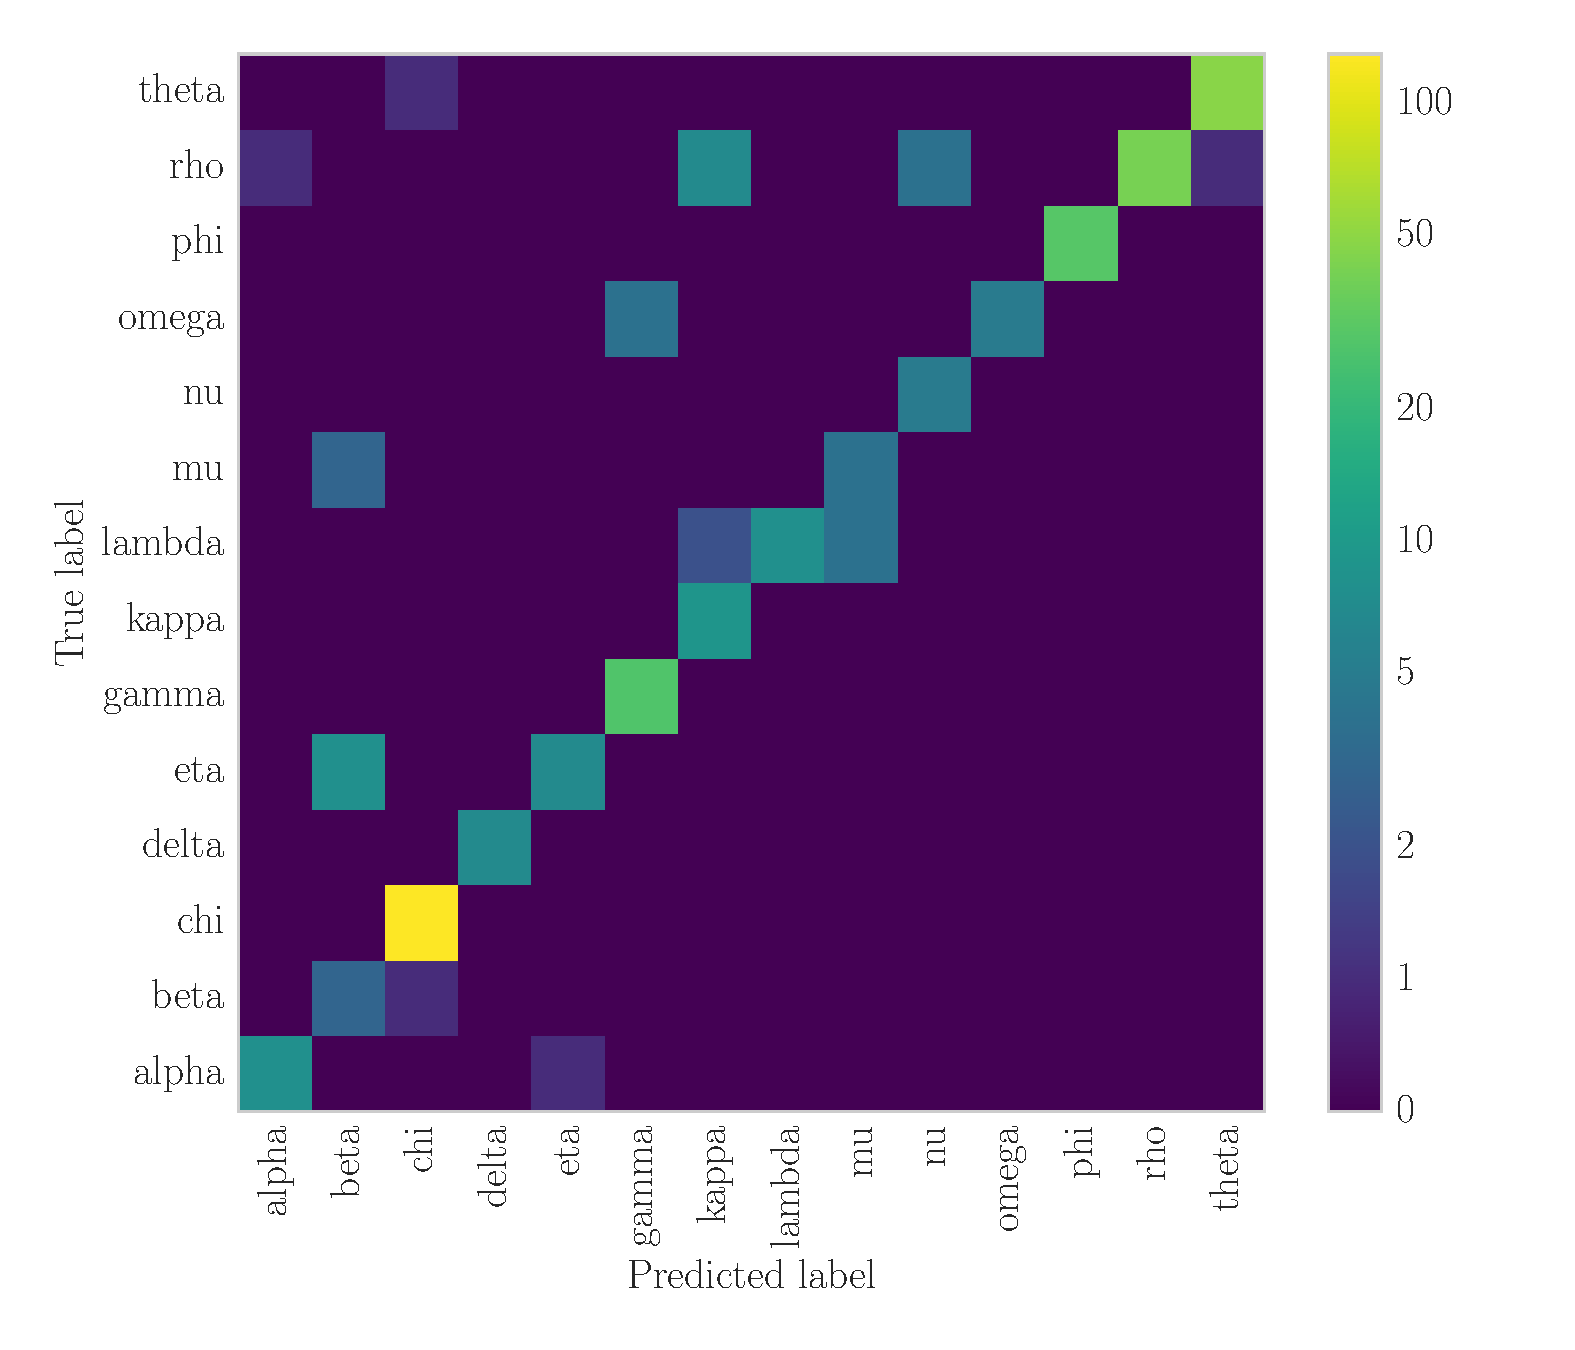
\includegraphics[width=9cm]{grs1915_supervised_cm.pdf}
\caption{Confusion matrix for the machine classification (x-axis) versus the human classification (assumed as the ``true label'') on the 
y-axis. On the diagonal are classes where the human and machine classifications agree. Off-diagonal cases occur where there is a 
disagreement.} 
\label{fig:confusion_matrix}
\end{center}
\end{figure}

The multinomial probability distribution used in the logistic regression model allows for calculating the predicted probability for each class and each sample. We compared the predicted probabilities for each human-generated class and computer-generated class for all of the confused cases and compared them to those cases where human and computer-generated classifications agree. While samples where human and computer agree show a very high predicted probability for the chosen class ($>0.9$ in more than $75\%$ of all cases), this is generally not the case for confused cases, where the predicted probability of the class chosen by the computer can be as small as $0.3$ and close to the human-generated class. Cases with the closest probabilities between human and computer-generated classes 
are more prevalent in second category laid out above. Conversely, for some confused cases, the predicted probability for the computer-generated class is very high, $>0.8$. These cases tend to be in the first and third category. 
 
\subsection{Overall Distribution of States}

In Figure \ref{fig:state_durations} we compare the total duration the source spent in each state during the observed intervals for both the human classified part of the data as well as the computer-generated classification. At the same time, this presents a split in time: \citet{belloni2000} and citet{kleinwolt2002} classified observations between 1996 June and 1999 December, with an additional state identified in an observation on 2003 Mar 6. Trained on these human classifications,
we allowed the computer to find classes for the remaining observations, spanning from $2000$ Jan to the end of \rxte's lifetime in early 2012. 
Assuming that the logistic regression model generally reproduces the human classification, one may then use the data set to search for time evolution in the overall pattern of states. 

\begin{figure}[htbp]
\begin{center}
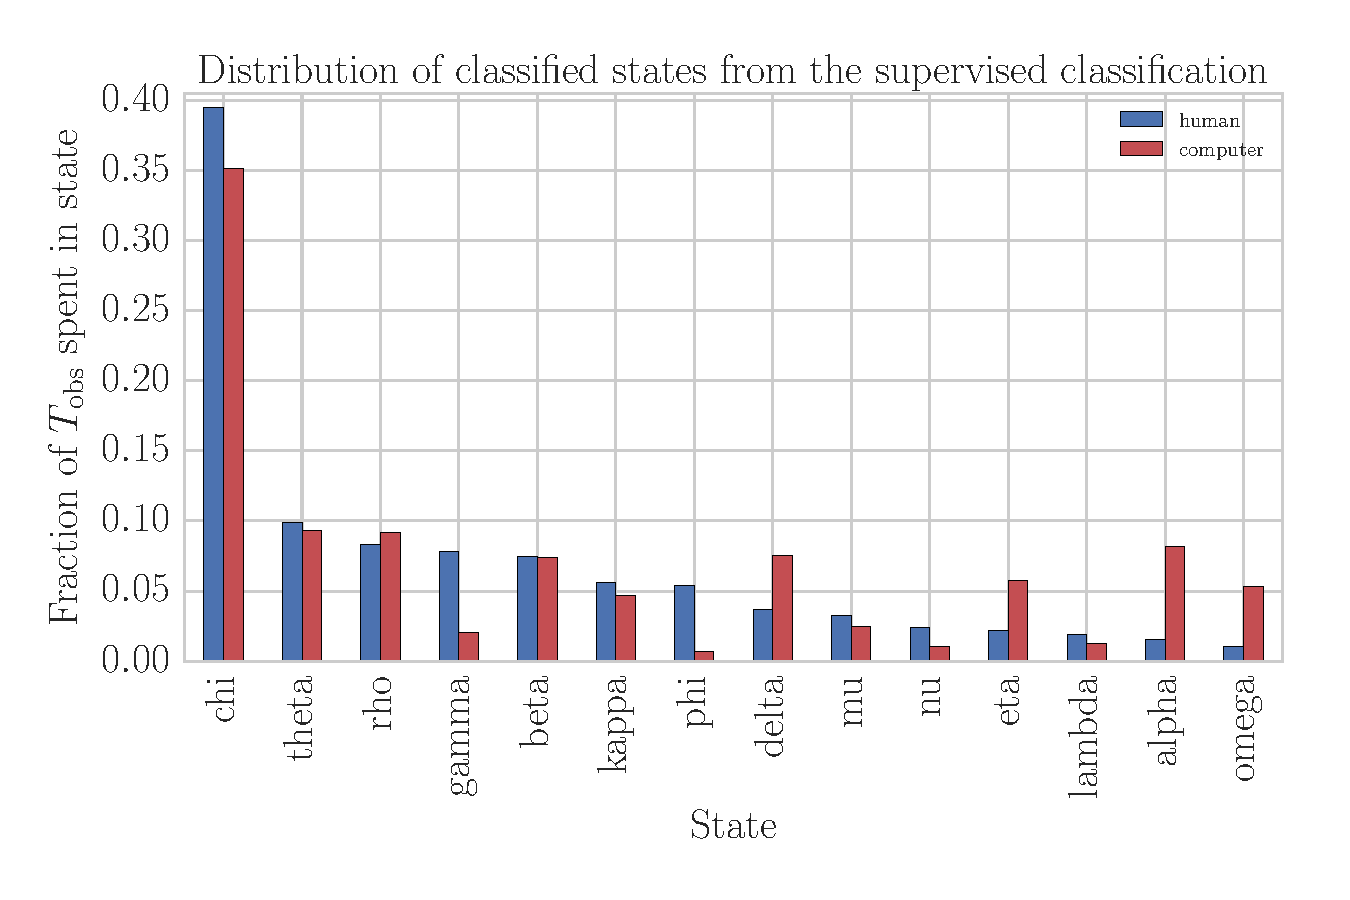
\includegraphics[width=9cm]{grs1915_supervised_states_histogram.pdf}
\caption{Fraction of total observation time $T_\mathrm{obs}$ assigned to a certain state in both the human-classified data (1996-$\sim\!\! 2000$; blue) and the machine-classified data ( $\sim\!\! 2000$ - 2011; red). Durations spent in each state are calculated from the human and computer-generated labels taking into 
account the overlap between segments for long observations.} 
\label{fig:state_durations}
\end{center}
\end{figure}

We find that broadly, the machine classification reproduces the human classification. Particularly the $\chi$ state remains the most common state to find GRS 1915+105 in. Other states such as $\beta$, $\kappa$, $\lambda$, $\mu$, $\rho$ and $\theta$ are represented similarly often, other classes occur with a significantly different frequency in later observations. It is important to note here that the prior on the state occurrences in the logistic regression model was based on the previous state occurrences, that is, a state with a higher previous occurrence was more probable to occur again than a state that was only seen once or twice. In this context, it is interesting to note the relatively higher fraction of time spent in the $\eta$ and $\omega$ states compared to the human-classified data set. 
This may, to some degree, be due to chance: with only one confirmed observation for each class, and the small fraction of the telescope spent on the source, it is intrinsically hard to reliably estimate the duration of the source previously spent in the source. Similar reasoning may be applied to the $\alpha$ state, though it is interesting that all states that are very rare during the initial four years of observations appear more commonly later, to a higher degree than perhaps originally expected. Conversely, the states $\gamma$ and $\phi$, relatively common during the initial four years, occur much less frequently during later observations.

Based on our results from Section \ref{sec:confusion}, it is unlikely that confused classes play a significant role in explaining the discrepancy between the state durations in the human and computer-classified data sets. Confusions seem to dominate in classes whose fraction of observation time are very similar. 
Additionally, classes such as $\eta$ and $\omega$ that are much more common in the computer-classified part of the data tend to be confused by the classifier with more common states, thus tend to loose observation time to these states. This means that perhaps the discrepancy between the early years of the current prolonged outburst of GRS 1915+105 and the later years is even more pronounced than our results indicate. 

For the classes with the strongest relative discrepancies---$\alpha$, $\eta$ and $\omega$---we also explored the probabilities of the assigned state in an 
effort to learn how certain the logistic regression model was in its classification for those states. We find that for states $\eta$ and $\alpha$, the classfier is 
fairly certain in its predictions: for example, for class $\eta$, more than $70\%$ of all classified samples have a probability for the source being in state $\eta$ that is 
$>0.8$, and for $88\%$ of all classified samples have a probability of $\eta$ being the true state that is at least twice that of the state with the second-largest 
probability. For this state, there is a small population of samples ($\sim 7\%$) that might be in state $\beta$, $\rho$ or $\theta$ with a probability of up to $0.4$, that is close to equally likely to the classification as $\eta$. 

Similar reasoning can be applied to class $\alpha$ with similar numbers, but not to class $\omega$, where the situation is much less clear.
Only $33\%$ of samples have a probability of $\omega$ being the true state of $>0.8$, indicating that for many samples, the probability for state $\omega$ is quite low. Indeed, for numerous samples the probability of class $\omega$ is close to that of the second-most probable state. The latter is dominated by class $\chi$, which is unsurprising, since segments of class $\chi$ with a high-count rate might mimic segments of class $\omega$ quite well, if they lack the characteristic dips of the latter state. However, an appreciable number of samples shows similar probabilities between class $\omega$ and classes $\theta$, $\beta$, $\rho$ and $\kappa$ as the second-most probable states. This is somewhat surprising, since the morphology of the latter states tends to be vastly more complex than class $\omega$, indicating perhaps once more that our simple heuristic models for the variability in the light curve are insufficient to capture the intricacies of the latter states correctly.

In summary, we conclude that the effect of an increased number of observations in states $\eta$ and $\alpha$ in the machine-classified data are likely real, while the increase in class $\omega$ may well be attributed to mis-classifications that are rooted in an inadequate model for the variability.
%% Note: maybe plot examples and look at them?

For states that are much less represented in the machine-classified data set compared to the original human classification, we explore whether these states might have lost samples due to mis-classification as well. For this, we found all samples where states $\phi$ and $\gamma$, both of which are almost not present in the 
machine-classified data set, were the second-most probable state, and compared their probability to that of the state the logistic regression model chose for these specific samples. We find that state $\phi$ comes often second to $\chi$-state observations, which is perhaps not surprising given the morphological similarities between the two states. However, because the hardness ratios are quite different for both states, we find that the logistic regression model assigns these samples to class $\chi$ with a very high degree of confidence (with a $\chi$-state probability of $>0.8$ in $>93\%$ of all samples where $\phi$ has the second-highest probability). This indicates that the paucity of $\phi$-state observations in recent years is likely real. 
For state $\gamma$, on the other hand, the situation is more complex. We find $\sim 200$ segments classified by our model as $\delta$-state observations, of which $\sim XX\%$ (CALCULATE VALUES) have a comparable probability of being state $\gamma$. This fraction is overall large enough to explain the drop in $\gamma$-state observations between the human- and the machine-classified data set.


% NEED PLOT: PCA decomposition with all states coloured in

\subsection{Time Evolution of States}
% NEED PLOT: transition matrix
% NEED PLOT: Time evolution of the states

% Look at time evolution + transition matrix: 
% - is there a "connecting" state that the source jumps in and out of?
% - do certain states always follow each other
% - are there cycles?
% Look at overall distribution of states versus training set: are the first four years representative of the long-term evolution?



\subsection{Supervised Classification with Physically Motivated Labels}

% Add "physical" classification based on chaotic versus deterministic classification
% - What does the source spend most of its time in?
% - Are there certain sequences of states appearing often? Are there certain states always following other states?
% - What classes do eta and omega most likely belong to?



\section{Discussion}
%% Note: Deliver classification of all observations online somewhere!

\subsection{Caveats and Limits}
% Caveats
% - Can only classify previously identified states
% - Relies on accuracy of human classification as "ground truth"

\section{Conclusion}

\paragraph{acknowledgements}

\bibliographystyle{apj}
\bibliography{grs1915_classification_paper}

\end{document}


